%!TEX root = ../../presentation.tex

\newcommand{\iconsize}{\fontsize{30pt}{30pt}\selectfont}

\tikzset{
  event/.style={
    draw,
    inner sep=0pt,
    circle,
    minimum width=4mm
  },
  events/.style={
    xscale=.8,
    yscale=.6
  },
  unit/.style={
    event,
    path picture={ 
      \draw[black]
        (path picture bounding box.south east) -- (path picture bounding box.north west)
        (path picture bounding box.south west) -- (path picture bounding box.north east);
    }
  },
  small unit/.style={
    unit,
    minimum width=2.5mm
  }
}

\chapter{Runtime Verification}
\label{chap_rv}
\targets{
  \item Understand runtime verification and the differences to other formal methods.
  \item Know when runtime verification is appropriate and helpful.
  \item Understand why and how we use LTL on finite words.
  \item Be able to write specifications in LTL.
}

\section{Runtime Verification}

\subsection{Validation}

\begin{frame}{Validation and Verification}
  \begin{Block}{Validation}
    \enquote{Are we building the right product?} \newline
    (Does the system meet the client’s expectations?)
  \end{Block}
  
  \begin{Block}{Verification}
    \enquote{Are we building the product right?} \newline
    (Does the system meet its specification?)
  \end{Block}
  
  \pause
  
  \only<presentation>{\vfill}
  
  \begin{definition}[Verification]
    Verification is comparing code with its specification.
  \end{definition}
\end{frame}

\begin{Frame}{Verification or Validation?}
  \begin{center}\LARGE
    Testing and Runtime Verification\\
    are \alert{verification techniques}.
  \end{center}

  \xxx\xxx

  \centerline{Both do not work if the specification is wrong.}
\end{Frame}

\subsection{Definition}

\begin{Frame}{Runtime Verification}
  \Large
  \alert{Verification technique} that allow for checking\\
  whether a \alert{run} of a system under scrutiny\\
  \alert{satisfies or violates} a given correctness property.

  \normalsize\vskip3ex\pause

  \hspace*{-2mm}
  \begin{tikzpicture}[node distance=3.5cm,on grid]
    \node[maincolor,label=below:Executable] (binary) {\iconsize\faCogs};
    \node[maincolor,label={[name=code label]below:Source Code},above=of binary] (code) {\iconsize\faFilesO};

    \path[very thick, maincolor, ->]
      (code label) edge[decorate, decoration=snake, shorten >=-3pt] (binary);

    \pause

    \node[examplecolor, right=3cm of code, label={[name=events label]below:Event Declaration}] (events) {\iconsize\faFileTextO};
    \node[examplecolor,right=1cm of binary, label={[label distance=-9pt]below right:\shortstack[l]{Event\\Generator}}] (observer) {\Huge\faCog};

    \path[very thick, examplecolor, ->]
      (events label) edge[decorate, decoration=snake, shorten >=-2pt] (observer);

    \pause

    \node[alertedcolor, right=3.5cm of events, label={[name=spec label,label distance=3pt]below:Specification}] (spec) {\fontsize{38pt}{38pt}\selectfont$\boldsymbol\phi$};
    \node[inner sep=0pt,draw=alertedcolor,very thick,regular polygon,regular polygon sides=6,fill=alertedcolor!18, right=5.5cm of observer, label={[label distance=5pt]below:Monitor}] (monitor) {$M^\phi$};
    \node[right=16mm of monitor, label={[label distance=.5pt]below:Verdict}] (verdict) {\LARGE\shortstack{\goodmark\\\badmark}};

    \path[very thick, alertedcolor, ->]
      (spec label) edge[decorate, decoration=snake] (monitor);    
    
    \node[event,fill=maincolor!18, right=2cm of observer] (e1) {$e_4$};
    \node[event,fill=maincolor!18, right=7mm of e1] (e2) {$e_3$};
    \node[event,fill=maincolor!18, right=7mm of e2, label={[label distance=12pt]below:Events}] (e3) {$e_2$};
    \node[event,fill=maincolor!18, right=7mm of e3] (e4) {$e_1$};
    \path[shorten >=0pt, thick]
      (observer) edge (e1)
      (e1) edge (e2)
      (e2) edge (e3)
      (e3) edge (e4);
    \path[thick, ->]
      (e4) edge (monitor)
      (monitor) edge (verdict);
  \end{tikzpicture}
\end{Frame}

\begin{frame}[t]{Run}
  \begin{center}
    \begin{tikzpicture}[
        on grid,
        auto,
        maincolor,
        shorten >=0pt,
        shorten <=0pt]
      \node[coordinate] (start) {};
      \node[coordinate, right=8em of start] (mid) {};
      \path[thick,->]
        (mid) edge node[below] {Run} +(8em,0);
      \path[thick]
        (start) edge (mid)
        (start) edge +(0,1ex)
                edge +(0,-1ex);
    \end{tikzpicture}
  \end{center}

  \begin{definition}[Run]
    A run of a system is a possibly infinite
    sequence of the system's states.
    Formally, a run may be considered as a possibly infinite
    \emph{word} or \emph{trace}.
  \end{definition}
  
  \begin{itemize}
    \item Runs are formed by current variable
    assignments,
    \item or as the sequence of actions a system is emitting or
    performing.
  \end{itemize}
\end{frame}

\begin{frame}[t]{Execution}
  \begin{center}
    \begin{tikzpicture}[
        on grid,
        auto,
        maincolor,
        shorten >=0pt,
        shorten <=0pt]
      \node[coordinate] (start) {};
      \node[coordinate, right=8em of start] (mid) {};
      \path[thick,->]
        (mid) edge node[below] {Run} +(8em,0);
      \path[thick, alertedcolor]
        (start) edge node[below] {Execution} (mid)
        (mid) edge +(0,1ex)
              edge +(0,-1ex)
        (start) edge +(0,1ex)
                edge +(0,-1ex);
    \end{tikzpicture}
  \end{center}

  \begin{definition}[Execution]
    An \emph{execution} of a system is a
    \emph{finite prefix} of a run and, formally, it is a finite
    trace.
  \end{definition}
  
  \begin{itemize}
    \item In verification, we check whether a
      run of a system adhere to given
      correctness properties.
    \item RV is primarily used on executions.
    \item A monitor checks whether an execution meets a correctness property. 
  \end{itemize}
\end{frame}

\begin{Frame}{RV and the Word Problem}
  A simple monitor outputs
  \begin{itemize}
    \item \alert{yes} if the execution satisfies the correctness property,
    \item \alert{no} if not.
  \end{itemize}
  
  \xxx
  
  \begin{itemize}
    \item Let $\sem{\phi}$ denote the set of valid executions given
      by property $\phi$.
    \item Then runtime verification answers the \alert{word problem}
      $w \in \sem{\phi}$.
    \item The word problem can be decided with lower
      complexity compared to the subset problem.
  \end{itemize}
\end{Frame}

\begin{Frame}{Monitoring the Execution of a System}
  We want to monitor the \alert{execution of a system}.
  
  \xxx

  We have already seen that
  \begin{itemize}
    \item A \alert{run} of a system is a possibly infinite sequence of the
      system's states.
    \item An \alert{execution} of a system is a \alert{finite prefix} of a run.
  \end{itemize}
  
  \xxx
  
  \begin{Block}{Observations}
    \begin{itemize}
      \item We describe the execution of a system in a \alert{discrete} way.
      \item The system is in exactly one state at a time.
      \item In the next step the system is in the next state.
    \end{itemize}
  \end{Block}
\end{Frame}

\begin{Frame}{Atomic Propositions}
  \begin{itemize}
    \item An atomic proposition is an indivisible bit.
    \item We consider a fixed set of finitely many such bits. 
    \item In every state every atomic proposition is either true or false.
    \item In other words:\\
      In every state of the execution some atomic propositions hold.
  \end{itemize}
  
  \begin{example}
    \begin{itemize}
      \item Variable \texttt{count} is greater than 5.
      \item Memory for a variable \texttt{data} is allocated.
      \item Memory for \texttt{data} is free.
      \item The file handle \texttt{logfile} points to an opened file.
    \end{itemize}
  \end{example}
\end{Frame}

\begin{Frame}{States}
  \begin{itemize}
    \item Let $\op{AP}$ be a fixed finite non empty set of atomic propositions.
    \item $\Sigma = 2^{\op{AP}}$ is the power set of these.
    \item A state can be seen as an element $a \in \Sigma$.
  \end{itemize}
\end{Frame}

\begin{Frame}{Propositions vs. Events}
  \begin{columns}
    \column{.5\textwidth}
      \textbf{\color{maincolor}Propositions}
      \begin{itemize}
        \item A state consist of\\
          a set of propisitions.
        \item A word $w \in (2^{\op{AP}})^\omega$ is\\
          a sequence of states.
        \item The formula $p \LTLand q$\\
          requires that $p$ and $q$\\
          hold in the current\\
          state and therefore\\
          can be fulfilled.
      \end{itemize}

    \column{.5\textwidth}
      \textbf{\color{maincolor}Events}
      \begin{itemize}
        \item A state consist of\\
          one event.
        \item A word $w \in (\op{EV})^\omega$ is\\
          a sequence of events.
        \item The formula $p \LTLand q$\\
          requires that the current\\
          state is $p$ and $q$\\
          and therefore \alert{cannot\\
          be fulfilled for $p \neq q$}!
      \end{itemize}
  \end{columns}
\end{Frame}

\subsection{Linear Temporal Logic}

\begin{Frame}{Specifying Correct Runs}
  \begin{itemize}
    \item Executions are words
    \item We specify behavior of correct runs $\phi$\\
      and want to check $w \in \sem{\phi}$
    \item We can use any formal description of words to specify $\phi$
    \begin{itemize}
      \item Set notation
      \item Regular expressions
      \item \alert<2>{Linear temporal logic (LTL)}
    \end{itemize}
  \end{itemize}
\end{Frame}

\begin{frame}{Monitoring Finite Executions Requires Finite LTL}
  \begin{itemize}
    \item Executions are \alert{finite} words\\
      Finite words always end
    \item $\LTLnot\LTLnext\phi \overset?\equiv \LTLnext\LTLnot\phi$
    \pause
    \item $\LTLfinally \LTLnot \LTLnext \LTLtrue$ is only fulfilled on finite words
    \item $\LTLfinally \LTLnext \LTLnot \LTLtrue$ is never fulfilled
  \end{itemize}

  \xxx\xxx\pause

  \begin{center}
    \begin{columns}
      \column{3.8cm}
      \inhead{infinite words}
      \begin{itemize}
        \item $\LTLnot\LTLnext\phi \equiv \LTLnext\LTLnot\phi$
        \item $\LTLglobally \phi \equiv \phi \LTLand \LTLnext\LTLglobally\phi$
        \item $\LTLfinally \phi \equiv \phi \LTLor \LTLnext\LTLfinally\phi$
      \end{itemize}
      \column{3.8cm}\pause
      \inhead{finite words}
      \begin{itemize}
        \item $\LTLnot\LTLnext\phi \equiv \alert{\LTLweaknext}\LTLnot\phi$
        \item $\LTLglobally \phi \equiv \phi \LTLand \alert{\LTLweaknext}\LTLglobally\phi$
        \item $\LTLfinally \phi \equiv \phi \LTLor \alert{\LTLnext}\LTLfinally\phi$
      \end{itemize}
    \end{columns}
  \end{center}
\end{frame}

\section{Using Runtime Verification}

\subsection{Comparison}

\newcommand{\cell}[1]{\parbox[t]{.4\textwidth}{\vskip-5pt\raggedright#1\strut\par\vskip3pt}}

\newcommand{\smallcompare}[6]{
  \def\tempa{#1}%
  \def\tempb{#2}%
  \def\tempc{#3}%
  \def\tempd{#4}%
  \def\tempe{#5}%
  \def\tempf{#6}%
  \begin{zebratabular}{ll}
    \headerrow \tempa \\
    \cell{\tempb} \\
    \cell{\tempc} \\
    \cell{\tempd} \\
    \cell{\tempe} \\
    \cell{\tempf}
  \end{zebratabular}
}

\newcommand{\compare}[6]{
  \def\tempa{#1}%
  \def\tempb{#2}%
  \def\tempc{#3}%
  \def\tempd{#4}%
  \def\tempe{#5}%
  \def\tempf{#6}%
  \comparecontinue
}

\newcommand{\comparecontinue}[6]{
  \begin{zebratabular}{ll}
    \headerrow \tempa & #1 \\
    \cell{\tempb}
    &\cell{#2} \\
    \cell{\tempc}
    &\cell{#3} \\
    \cell{\tempd}
    &\cell{#4} \\
    \cell{\tempe}
    &\cell{#5} \\
    \cell{\tempf}
    &\cell{#6}
  \end{zebratabular}}

\begin{Frame}{Testing}
\begin{center}
  \smallcompare
    {Testing}
    {$i_0/o_0, i_1/o_1, \ldots \to S$}
    {Does system $S$ satisfy the \alert{input/output sequence}
             $i_0/o_0, i_1/o_1, \ldots$?\\}
    {Input/output sequence is written \alert{manually}.\\}
    {Main research topic is \alert{input/output sequence generation}.}
    {\alert{Current execution} must be correct.}
    
\end{center}
\end{Frame}

\begin{Frame}{Testing vs. Oracle Testing}
\begin{center}
  \compare
    {Testing}
    {$i_0/o_0, i_1/o_1, \ldots \to S$}
    {Does system $S$ satisfy the \alert{input/output sequence}
             $i_0/o_0, i_1/o_1, \ldots$?\\}
    {Input/output sequence is written \alert{manually}.}
    {Main research topic is \alert{input/output sequence generation}.}
    {\alert{Current execution} must be correct.}
    %----------%
    {Oracle Testing}
    {$i_0, i_1, \ldots \to S \times M$}
    {Does system $S$ satisfy the \alert{test oracle} $M$ on input sequence
             $i_0, i_1, \ldots$?}
    {Input sequence and test oracle are written \alert{manually}.}
    {Main research topic is \alert{input sequence generation}.}
    {\alert{Current execution} must be correct.}

\end{center}
\end{Frame}

\begin{Frame}{Oracle Testing vs. Runtime Verification}
\begin{center}
  \compare
    {Oracle Testing}
    {$i_0, i_1, \ldots \to S \times M$}
    {Does system $S$ satisfy the \alert{test oracle} $M$ on input sequence
             $i_0, i_1, \ldots$?\\}
    {Input sequence and test oracle are written \alert{manually}.}
    {Main research topic is \alert{input sequence generation}.}
    {\alert{Current execution} must be correct.}
    %----------%
    {Runtime Verification}
    {$i_0,i_1,\ldots \to S \times M_\phi$}
    {Does system $S$ satisfy the \alert{generated monitor}
      $M_\phi$ on input sequence $i_0, i_1, \ldots$?}
    {Monitor is \alert{synthesized} from correctness property.}
    {Main research topic is \alert{monitor generation}.}
    {\alert{Current execution} must be correct.}
\end{center}
\end{Frame}

\begin{Frame}{Runtime Verification vs. Model Checking}
\begin{center}
  \compare
    {Runtime Verification}
    {$i_0,i_1,\ldots \to S \times M_\phi$}
    {Does system $S$ satisfy the \alert{generated monitor}
      $M_\phi$ on input sequence $i_0, i_1, \ldots$?\\}
    {Monitor is \alert{synthesized} from correctness property.}
    {Main research topic is \alert{monitor generation}.}
    {\alert{Current execution} must be correct.}
    %----------%
    {Model Checking}
    {$S \models \phi$ via $\mathcal L(S) \subseteq \mathcal L(\phi)$}
    {Is system $S$ a \alert{model of the correctness property} $\phi$?
         Are all runs of the system $\mathcal L(S)$ a subset of all
         correct runs $\mathcal L(\phi)$?}
    {\alert{Automatic proof} using manually created system model.}
    {Main research topic are \alert{algorithms for proving model relation}.}
    {\alert{All runs} must be correct.}
\end{center}
\end{Frame}

\begin{Frame}{Model Checking vs. Theorem Proofing}
\begin{center}
  \compare
    {Model Checking}
    {$S \models \phi$ via $\mathcal L(S) \subseteq \mathcal L(\phi)$}
    {Is system $S$ a \alert{model of the correctness property} $\phi$?
         Are all runs of the system $\mathcal L(S)$ a subset of all
         correct runs $\mathcal L(\phi)$?}
    {\alert{Automatic proof} using manually created system model.}
    {Main research topic are \alert{algorithms for proving model relation}.}
    {\alert{All runs} must be correct.}
    %----------%
    {Theorem Proving}
    {$S \models \phi$ via $S \vdash \phi$}
    {Is system $S$ a \alert{model of the correctness property} $\phi$?
         Can we find a proof that property $\phi$
         derives from system $S$?}
    {Proof is done \alert{manually} by deriving property from the system.}
    {Main research topic is \alert{proof generation using a calculus}.}
    {\alert{All runs} must be correct.}
\end{center}
\end{Frame}

\renewcommand{\cell}[2]{\parbox[c]{#1}{\vskip3pt\centering#2\strut\par}}

\begin{frame}{Conclusion of the Comparison}
  \begin{center}
  \begin{zebratabular}{cccc}
    \headerrow SST & RV & MC & TP \\
    \cell{5em}{$I/O \to S$ \\ resp. \\ $I \to S \times M$}
    &\cell{5em}{$I \to S \times M_\phi$}
    &\cell{6em}{$S \models \phi$ \\ via \\ $\mathcal L(S) \subseteq \mathcal L(\phi)$}
    &\cell{4em}{$S \models \phi$ \\ via \\ $S \vdash \phi$} \\
    \cell{5em}{sequence generation}
    &\cell{5em}{monitor synthesis}
    &\cell{6em}{proof algorithms}
    &\cell{4em}{manual proofs} \\
    \cell{5em}{current execution}
    &\cell{5em}{current execution}
    &\cell{6em}{all runs}
    &\cell{4em}{all runs}
  \end{zebratabular}
  \end{center}
  \vskip3ex
  \begin{itemize}
    \item input sequence $I = i_0, i_1, \ldots$
    \item output sequence $O = o_0, o_1, \ldots$
    \item system $S$
    \item test oracle resp. monitor $M$
    \item correctness property $\phi$
  \end{itemize}
\end{frame}

\subsection{Online Monitoring}

\begin{Frame}[fragile,t]{Examples of Evaluating Growing Words}
  Consider
  \begin{itemize}
    \item the alphabet $\Sigma = 2^{\op{AP}}$ where $\op{AP}=\{p,q\}$ and
    \item the properties $\phi = \LTLglobally p$ \qquad and $\phi' = \LTLfinally p$.
  \end{itemize}

  \xxx
  
  Lets watch monitors for RV at work:
  
  \begin{columns}
    \column{.5\textwidth}
    
      \begin{center}
        \makebox(120,120)[t]{
        \begin{tikzpicture}[
            every node/.style={
              inner sep=0pt
            },
            /tikz/ampersand replacement=\&
          ]
          \matrix[column sep=1ex] {
            \node {$w = $};
            \& \node (s1) {$\{p,q\}$};
            \& \uncover<2->{\node (s2) {$\{p\}$};}
            \& \uncover<3->{\node (s3) {$\{q\}$};}
            \& \uncover<4->{\node (s4) {$\{p\}$};} \\
          };
          
          \draw[examplecolor,thick,transform canvas={yshift=-.5em}]
            (s1.south west) edge[serif cm-serif cm] node[below=.3em]
              {$\top$} (s1.south east);
          \uncover<2->{\draw[examplecolor,thick,transform canvas={yshift=-2.5em}]
            (s1.south west) edge[serif cm-serif cm] node[below=.3em]
              {$\top$} (s2.south east);}
          \uncover<3->{\draw[alertedcolor,thick,transform canvas={yshift=-4.5em}]
            (s1.south west) edge[serif cm-serif cm] node[below=.3em]
              {$\bot$} (s3.south east);}
          \uncover<4->{\draw[alertedcolor,thick,transform canvas={yshift=-6.5em}]
            (s1.south west) edge[serif cm-serif cm] node[below=.3em]
              {$\bot$} (s4.south east);}
        \end{tikzpicture}
        }
      \end{center}
    \column{.5\textwidth}
      \begin{center}
        \makebox(120, 120)[t]{
        \begin{tikzpicture}[
            every node/.style={
              inner sep=0pt
            },
            /tikz/ampersand replacement=\&
          ]
          \matrix[column sep=1ex] {
            \uncover<5->{\node {$w' = $};}
            \& \uncover<5->{\node (s1) {$\{q\}$};}
            \& \uncover<6->{\node (s2) {$\{q\}$};}
            \& \uncover<7->{\node (s3) {$\{p,q\}$};}
            \& \uncover<8->{\node (s4) {$\{p\}$};} \\
          };
          
          \uncover<5->{\draw[alertedcolor,thick,transform canvas={yshift=-.5em}]
            (s1.south west) edge[serif cm-serif cm] node[below=.3em]
              {$\bot$} (s1.south east);}
          \uncover<6->{\draw[alertedcolor,thick,transform canvas={yshift=-2.5em}]
            (s1.south west) edge[serif cm-serif cm] node[below=.3em]
              {$\bot$} (s2.south east);}
          \uncover<7->{\draw[examplecolor,thick,transform canvas={yshift=-4.5em}]
            (s1.south west) edge[serif cm-serif cm] node[below=.3em]
              {$\top$} (s3.south east);}
          \uncover<8->{\draw[examplecolor,thick,transform canvas={yshift=-6.5em}]
            (s1.south west) edge[serif cm-serif cm] node[below=.3em]
              {$\top$} (s4.south east);}
        \end{tikzpicture}
}
      \end{center}
  \end{columns}
\end{Frame}

\begin{Frame}[fragile]{Impartiality}
  \begin{center}
    What are the \emph{relevant} outputs of my monitor?
  \end{center}

  \begin{block}{Be Impartial!}
    \begin{itemize}
      \item go for a final verdict (yes or no)
        only if you really know
      \item stick to your word!
    \end{itemize}
  \end{block}
  
  \vskip1ex
  
  \begin{definition}<presentation>[Impartiality]
    Impartiality requires that a finite trace is not evaluated to
    true or, respectively false, if there still exists an
    (possibly infinite) continuation leading to another verdict.
  \end{definition}
\end{Frame}

\begin{Frame}{We need Four-Valued Semantics}
  With
  \[ \mathbb B = \{\bot, \top\} \]
  we cannot be specific enough.

  \xxx

  We need
  \[ \mathbb B = \{\bot, \bot^c, \top^c, \top\} \]
  to distinguish between
  \begin{itemize}
    \item final verdicts (no further changes) and\\
    \item current verdicts (subject to change).
  \end{itemize}
\end{Frame}

\begin{Frame}[fragile,t]{Examples of Four-Valued Runtime Verification}
  Consider again
  \begin{itemize}
    \item the alphabet $\Sigma = 2^{\op{AP}}$ where $\op{AP}=\{p,q\}$ and
    \item the properties $\phi = \LTLglobally p$ \qquad and $\phi' = \LTLfinally p$.
  \end{itemize}
  
  Lets watch \emph{four-valued monitors} for RV at work:
  
  \begin{columns}
    \column{.5\textwidth}
    
      \begin{center}
        \makebox(120,120)[t]{
        \begin{tikzpicture}[
            every node/.style={
              inner sep=0pt
            },
            /tikz/ampersand replacement=\&
          ]
          \matrix[column sep=1ex] {
            \node {$w = $};
            \& \node (s1) {$\{p,q\}$};
            \& \uncover<2->{\node (s2) {$\{p\}$};}
            \& \uncover<3->{\node (s3) {$\{q\}$};}
            \& \uncover<4->{\node (s4) {$\{p\}$};} \\
          };
          
          \draw[orange,thick,transform canvas={yshift=-.5em}]
            (s1.south west) edge[serif cm-serif cm] node[below=.3em]
              {$\top^c$} (s1.south east);
          \uncover<2->{\draw[orange,thick,transform canvas={yshift=-2.5em}]
            (s1.south west) edge[serif cm-serif cm] node[below=.3em]
              {$\top^c$} (s2.south east);}
          \uncover<3->{\draw[alertedcolor,thick,transform canvas={yshift=-4.5em}]
            (s1.south west) edge[serif cm-serif cm] node[below=.3em]
              {$\bot$} (s3.south east);}
          \uncover<4->{\draw[alertedcolor,thick,transform canvas={yshift=-6.5em}]
            (s1.south west) edge[serif cm-serif cm] node[below=.3em]
              {$\bot$} (s4.south east);}
        \end{tikzpicture}
        }
      \end{center}
    \column{.5\textwidth}
      \begin{center}
        \makebox(120, 120)[t]{
        \begin{tikzpicture}[
            every node/.style={
              inner sep=0pt
            },
            /tikz/ampersand replacement=\&
          ]
          \matrix[column sep=1ex] {
            \uncover<5->{\node {$w' = $};}
            \& \uncover<5->{\node (s1) {$\{q\}$};}
            \& \uncover<6->{\node (s2) {$\{q\}$};}
            \& \uncover<7->{\node (s3) {$\{p,q\}$};}
            \& \uncover<8->{\node (s4) {$\{p\}$};} \\
          };
          
          \uncover<5->{\draw[orange,thick,transform canvas={yshift=-.5em}]
            (s1.south west) edge[serif cm-serif cm] node[below=.3em]
              {$\bot^c$} (s1.south east);}
          \uncover<6->{\draw[orange,thick,transform canvas={yshift=-2.5em}]
            (s1.south west) edge[serif cm-serif cm] node[below=.3em]
              {$\bot^c$} (s2.south east);}
          \uncover<7->{\draw[examplecolor,thick,transform canvas={yshift=-4.5em}]
            (s1.south west) edge[serif cm-serif cm] node[below=.3em]
              {$\top$} (s3.south east);}
          \uncover<8->{\draw[examplecolor,thick,transform canvas={yshift=-6.5em}]
            (s1.south west) edge[serif cm-serif cm] node[below=.3em]
              {$\top$} (s4.south east);}
        \end{tikzpicture}
}
      \end{center}
  \end{columns}
\end{Frame}

\subsection{Generating Traces}

\begin{frame}[label=current]{How To Get a Trace?}
  \begin{itemize}
    \item<2-> \alert<2>{Log File Analysis} (offline)\only<3->{, \alert<3>{Logging API} (online)}
    \item<4-> \alert<4>{Source Code Instrumentation}\only<5->{, \alert<5>{Binary Instrumentation}}
    \item<6-> \alert<6>{Tracing Tools / Debugger} (less intrusive)
    \item<7-> \alert<7>{Tracing Hardware} (non-intrusive)
  \end{itemize}

  \xxx

  \begin{tikzpicture}
    \node[maincolor,label={[name=code label]below:Source Code}] (code) {\iconsize\faFilesO};
    \node[maincolor,label=below:Executable, right=2.5cm of code] (binary) {\iconsize\faCogs};
    \path[very thick, maincolor, ->]
      (code) edge[decorate, decoration={snake, pre length=5pt, post length=3pt}, shorten >=-1pt] (binary);

    \uncover<4>{
      \node[alertedcolor, right=-5.5mm of code] {\huge\faPencil};}
    \uncover<5->{
      \node[right=-5.5mm of code] {\huge\faPencil};}
    \uncover<5>{
      \node[alertedcolor, above left=-8mm and -7mm of binary] {\huge\reflectbox\faPencil};}
    \uncover<6->{
      \node[above left=-8mm and -7mm of binary] {\huge\reflectbox\faPencil};}

    \begin{pgfonlayer}{background}
      \uncover<7->{
        \node[fit=(binary), thick, draw=maincolor, fill=maincolor!9, inner sep=38pt, label=below:Processor] (computer) {};}
      \uncover<6->{
        \node[fit=(binary), thick, draw=maincolor, fill=maincolor!18, inner sep=18pt, label=below:Runtime Environment] (rte) {};}
    \end{pgfonlayer}

    \node[inner sep=0pt,draw=alertedcolor,very thick,regular polygon,regular polygon sides=6,fill=alertedcolor!18, below right=0cm and 2.5cm of binary, label={[label distance=5pt]below:Monitor}] (monitor) {$M^\phi$};

    \uncover<2->{
      \node[above=1.5cm of monitor, maincolor, label={[name=log label]below:Event Log}] (log) {\iconsize\faList};}

    \uncover<2>{
      \path[very thick, alertedcolor] (binary) edge[shorten <=-3pt, ->, out=45, in=180] (log);
      \path[very thick, alertedcolor] (log label) edge[->] (monitor);}
    \uncover<3->{
      \path[very thick] (binary) edge[shorten <=-3pt, ->, out=45, in=180] (log);
      \path[very thick] (log label) edge[->] (monitor);}

    \uncover<3>{
      \path[very thick, alertedcolor] (binary) edge[shorten <=-3pt, ->, out=0,in=150] (monitor);}
    \uncover<4->{
      \path[very thick] (binary) edge[shorten <=-3pt, ->, out=0,in=150] (monitor);}

    \uncover<6>{
      \path[very thick, alertedcolor] ($(rte.east) - (0,.8)$) edge[->, out=0, in=180] (monitor);}
    \uncover<7->{
      \path[very thick] ($(rte.east) - (0,.8)$) edge[->, out=0, in=180] (monitor);}

    \uncover<7>{
      \path[very thick, alertedcolor] ($(computer.east) - (0,1.5)$) edge[->, out=0,in=210] (monitor);}
  \end{tikzpicture}
\end{frame}

\section{Writing LTL Specifications}

\subsection{LTL Patterns}

\begin{Frame}[t]{LTL Patterns}
  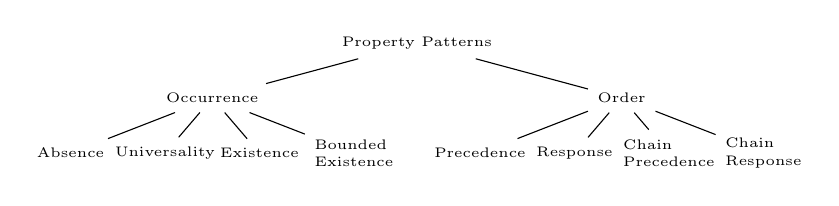
\begin{tikzpicture}[
      level 1/.style={sibling distance=5.2cm},
      level 2/.style={sibling distance=1.2cm},
      level distance=.7cm,
      alert/.style={alertedcolor, font=\tiny\bfseries},
      normal/.style={black, font=\tiny}]
    \node[normal] {Property Patterns}
      child { node[normal] {Occurrence}
        child { node[normal] {Absence} }
        child { node[normal] {Universality} }
        child { node[normal] {Existence} }
        child { node[normal] {\shortstack[l]{Bounded\\Existence}} }
      }
      child { node[normal] {Order}
        child { node[normal] {Precedence} }
        child { node[normal] {Response} }
        child { node[normal] {\shortstack[l]{Chain\\Precedence}} }
        child { node[normal] {\shortstack[l]{Chain\\Response}} }
      };
  \end{tikzpicture}

  \xxx\xxx

  \scriptsize
  \begin{thebibliography}{12}
    \bibitem{}
    Matthew B. Dwyer, George S. Avrunin, James C. Corbett:
    \newblock
    Property specification patterns for finite-state verification.
    \newblock
    Second Workshop on Formal Methods in Software Practice 1998: 7--15
    \newblock
    \emph{This paper gives an introduction to the patterns system.}

    \bibitem{}
    Matthew B. Dwyer, George S. Avrunin, James C. Corbett:
    \newblock
    Patterns in Property Specifications for Finite-State Verification.
    \newblock
    International Conference on Software Engineering 1999: 411--420
    \newblock
    \emph{This paper describes a survey of property specifications, and presents the results of the survey.}
  \end{thebibliography}
\end{Frame}

\begin{Frame}[t]{LTL Patterns: Absence}
  \begin{tikzpicture}[
      level 1/.style={sibling distance=5.2cm},
      level 2/.style={sibling distance=1.2cm},
      level distance=.7cm,
      alert/.style={alertedcolor, font=\tiny\bfseries},
      normal/.style={black, font=\tiny}]
    \node[alert] {Property Patterns}
      child { node[alert] {Occurrence} edge from parent[alert]
        child { node[alert] {Absence} edge from parent[alert] }
        child { node[normal] {Universality} edge from parent[normal] }
        child { node[normal] {Existence} edge from parent[normal] }
        child { node[normal] {\shortstack[l]{Bounded\\Existence}} edge from parent[normal] }
      }
      child { node[normal] {Order}
        child { node[normal] {Precedence} }
        child { node[normal] {Response} }
        child { node[normal] {\shortstack[l]{Chain\\Precedence}} }
        child { node[normal] {\shortstack[l]{Chain\\Response}} }
      };
  \end{tikzpicture}

  \xxx

  \begin{block}{Intent}
    To describe a portion of a system's execution that is free of certain events or states. Also known as Never.\\\strut
  \end{block}

  \xxx

  \[ \LTLglobally \LTLnot p \]

  \xxx

  \centering
  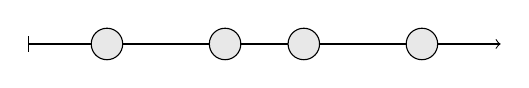
\begin{tikzpicture}[shorten >=0pt]
    \node[event, fill=gray!18] at (1,0) (x1) {};
    \node[event, fill=gray!18] at (2.5,0) (x2) {};
    \node[event, fill=gray!18] at (3.5,0) (x3) {};
    \node[event, fill=gray!18] at (5,0) (x4) {};
    \path
      (0,0) edge[|-]
      (x1) (x1) edge (x2) (x2) edge (x3) (x3) edge (x4) (x4) edge[->] +(1,0);
  \end{tikzpicture}
\end{Frame}

\begin{Frame}[t]{LTL Patterns: Universality}
  \begin{tikzpicture}[
      level 1/.style={sibling distance=5.2cm},
      level 2/.style={sibling distance=1.2cm},
      level distance=.7cm,
      alert/.style={alertedcolor, font=\tiny\bfseries},
      normal/.style={black, font=\tiny}]
    \node[alert] {Property Patterns}
      child { node[alert] {Occurrence} edge from parent[alert]
        child { node[normal] {Absence} edge from parent[normal] }
        child { node[alert] {Universality} edge from parent[alert] }
        child { node[normal] {Existence} edge from parent[normal] }
        child { node[normal] {\shortstack[l]{Bounded\\Existence}} edge from parent[normal] }
      }
      child { node[normal] {Order}
        child { node[normal] {Precedence} }
        child { node[normal] {Response} }
        child { node[normal] {\shortstack[l]{Chain\\Precedence}} }
        child { node[normal] {\shortstack[l]{Chain\\Response}} }
      };
  \end{tikzpicture}

  \xxx

  \begin{block}{Intent}
    To describe a portion of a system's execution which contains only states that have a desired property. Also known as Henceforth and Always.\strut
  \end{block}

  \xxx

  \[ \LTLglobally p \]

  \xxx

  \centering
  \begin{tikzpicture}[shorten >=0pt]
    \node[event, fill=maincolor!18] at (1,0) (x1) {$p$};
    \node[event, fill=maincolor!18] at (2.5,0) (x2) {$p$};
    \node[event, fill=maincolor!18] at (3.5,0) (x3) {$p$};
    \node[event, fill=maincolor!18] at (5,0) (x4) {$p$};
    \path
      (0,0) edge[|-]
      (x1) (x1) edge (x2) (x2) edge (x3) (x3) edge (x4) (x4) edge[->] +(1,0);
  \end{tikzpicture}
\end{Frame}

\begin{Frame}[t]{LTL Patterns: Existence}
  \begin{tikzpicture}[
      level 1/.style={sibling distance=5.2cm},
      level 2/.style={sibling distance=1.2cm},
      level distance=.7cm,
      alert/.style={alertedcolor, font=\tiny\bfseries},
      normal/.style={black, font=\tiny}]
    \node[alert] {Property Patterns}
      child { node[alert] {Occurrence} edge from parent[alert]
        child { node[normal] {Absence} edge from parent[normal] }
        child { node[normal] {Universality} edge from parent[normal] }
        child { node[alert] {Existence} edge from parent[alert] }
        child { node[normal] {\shortstack[l]{Bounded\\Existence}} edge from parent[normal] }
      }
      child { node[normal] {Order}
        child { node[normal] {Precedence} }
        child { node[normal] {Response} }
        child { node[normal] {\shortstack[l]{Chain\\Precedence}} }
        child { node[normal] {\shortstack[l]{Chain\\Response}} }
      };
  \end{tikzpicture}

  \xxx

  \begin{block}{Intent}
    To describe a portion of a system's execution that contains an instance of certain events or states. Also known as Eventually.\strut
  \end{block}

  \xxx

  \[ \LTLfinally p \]

  \xxx

  \centering
  \begin{tikzpicture}[shorten >=0pt]
    \node[event, fill=gray!18] at (1,0) (x1) {};
    \node[event, fill=gray!18] at (2.5,0) (x2) {};
    \node[event, fill=maincolor!18] at (3.5,0) (x3) {$p$};
    \node[event, fill=gray!18] at (5,0) (x4) {};
    \path
      (0,0) edge[|-]
      (x1) (x1) edge (x2) (x2) edge (x3) (x3) edge (x4) (x4) edge[->] +(1,0);
  \end{tikzpicture}
\end{Frame}

\begin{Frame}[t]{LTL Patterns: Bounded Existence}
  \begin{tikzpicture}[
      level 1/.style={sibling distance=5.2cm},
      level 2/.style={sibling distance=1.2cm},
      level distance=.7cm,
      alert/.style={alertedcolor, font=\tiny\bfseries},
      normal/.style={black, font=\tiny}]
    \node[alert] {Property Patterns}
      child { node[alert] {Occurrence} edge from parent[alert]
        child { node[normal] {Absence} edge from parent[normal] }
        child { node[normal] {Universality} edge from parent[normal] }
        child { node[normal] {Existence} edge from parent[normal] }
        child { node[alert] {\shortstack[l]{Bounded\\Existence}} edge from parent[alert] }
      }
      child { node[normal] {Order}
        child { node[normal] {Precedence} }
        child { node[normal] {Response} }
        child { node[normal] {\shortstack[l]{Chain\\Precedence}} }
        child { node[normal] {\shortstack[l]{Chain\\Response}} }
      };
  \end{tikzpicture}

  \xxx

  \begin{block}{Intent}
    To describe a portion of a system's execution that contains \emph{at most} a specified number of instances of a designated state transition or event.\strut
  \end{block}

  \xxx

  \[ (\LTLnot p \LTLweakuntil (p \LTLweakuntil (\LTLnot p \LTLweakuntil (p \LTLweakuntil \LTLglobally \LTLnot p)))) \]

  \xxx

  \centering
  \begin{tikzpicture}[shorten >=0pt, every label/.style={maincolor}]
    \node[event, fill=gray!18] at (1,0) (x1) {};
    \node[event, fill=maincolor!18, label=below:1] at (2.5,0) (x2) {$p$};
    \node[event, fill=maincolor!18] at (3.5,0) (x3) {$p$};
    \node[event, fill=gray!18] at (5,0) (x4) {};
    \node[event, fill=maincolor!18, label=below:2] at (6,0) (x5) {$p$};
    \node[event, fill=gray!18] at (7.5,0) (x6) {};
    \path
      (0,0) edge[|-]
      (x1) (x1) edge (x2) (x2) edge (x3) (x3) edge (x4) (x4) edge (x5) (x5) edge (x6) (x6) edge[->] +(1,0);
  \end{tikzpicture}
\end{Frame}

\begin{Frame}[t]{LTL Patterns: Precedence}
  \begin{tikzpicture}[
      level 1/.style={sibling distance=5.2cm},
      level 2/.style={sibling distance=1.2cm},
      level distance=.7cm,
      alert/.style={alertedcolor, font=\tiny\bfseries},
      normal/.style={black, font=\tiny}]
    \node[alert] {Property Patterns}
      child { node[normal] {Occurrence}
        child { node[normal] {Absence} }
        child { node[normal] {Universality} }
        child { node[normal] {Existence} }
        child { node[normal] {\shortstack[l]{Bounded\\Existence}} }
      }
      child { node[alert] {Order} edge from parent[alert]
        child { node[alert] {Precedence} edge from parent[alert] }
        child { node[normal] {Response} edge from parent[normal] }
        child { node[normal] {\shortstack[l]{Chain\\Precedence}} edge from parent[normal] }
        child { node[normal] {\shortstack[l]{Chain\\Response}} edge from parent[normal] }
      };
  \end{tikzpicture}

  \xxx

  \begin{block}{Intent}
    To describe relationships between a pair of events/states where the occurrence of the first is a necessary pre-condition for an occurrence of the second.\strut
  \end{block}

  \xxx

  \[ \LTLnot p \LTLweakuntil s \]

  \xxx

  \centering
  \begin{tikzpicture}
    \node[event, fill=gray!18] at (1,0) (x1) {};
    \node[event, fill=examplecolor!18] at (2.5,0) (x2) {$s$};
    \node[event, fill=gray!18] at (3.5,0) (x3) {};
    \node[event, fill=maincolor!18] at (5,0) (x4) {$p$};
    \node[event, fill=gray!18] at (6,0) (x5) {};
    \node[event, fill=maincolor!18] at (7.5,0) (x6) {$p$};
    \path[shorten >=0pt]
      (0,0) edge[|-]
      (x1) (x1) edge (x2) (x2) edge (x3) (x3) edge (x4) (x4) edge (x5) (x5) edge (x6) (x6) edge[->] +(1,0);
    \draw[maincolor, ->, rounded corners=3pt]
      (x4) -- +(0,-.5) -| (x2);
    \draw[maincolor, ->, rounded corners=3pt]
      (x6) -- +(0,-.5) -| node[below, pos=.25] {$s$ must precede $p$} (x2);
  \end{tikzpicture}
\end{Frame}

\begin{Frame}[t]{LTL Patterns: Response}
  \begin{tikzpicture}[
      level 1/.style={sibling distance=5.2cm},
      level 2/.style={sibling distance=1.2cm},
      level distance=.7cm,
      alert/.style={alertedcolor, font=\tiny\bfseries},
      normal/.style={black, font=\tiny}]
    \node[alert] {Property Patterns}
      child { node[normal] {Occurrence}
        child { node[normal] {Absence} }
        child { node[normal] {Universality} }
        child { node[normal] {Existence} }
        child { node[normal] {\shortstack[l]{Bounded\\Existence}} }
      }
      child { node[alert] {Order} edge from parent[alert]
        child { node[normal] {Precedence} edge from parent[normal] }
        child { node[alert] {Response} edge from parent[alert] }
        child { node[normal] {\shortstack[l]{Chain\\Precedence}} edge from parent[normal] }
        child { node[normal] {\shortstack[l]{Chain\\Response}} edge from parent[normal] }
      };
  \end{tikzpicture}

  \xxx

  \begin{block}{Intent}
    To describe cause-effect relationships between a pair of events/states. An occurrence of the first, the cause, must be followed by an occurrence of the second, the effect.\strut
  \end{block}

  \xxx

  \[ \LTLglobally(p \LTLimp \LTLfinally s) \]

  \xxx

  \centering
  \begin{tikzpicture}
    \node[event, fill=gray!18] at (1,0) (x1) {};
    \node[event, fill=maincolor!18] at (2.5,0) (x2) {$p$};
    \node[event, fill=gray!18] at (3.5,0) (x3) {};
    \node[event, fill=maincolor!18] at (5,0) (x4) {$p$};
    \node[event, fill=gray!18] at (6,0) (x5) {};
    \node[event, fill=examplecolor!18] at (7.5,0) (x6) {$s$};
    \path[shorten >=0pt]
      (0,0) edge[|-]
      (x1) (x1) edge (x2) (x2) edge (x3) (x3) edge (x4) (x4) edge (x5) (x5) edge (x6) (x6) edge[->] +(1,0);
    \draw[maincolor, ->, rounded corners=3pt]
      (x2) -- +(0,-.5) -| node[below, pos=.25] {$p$ must be followed by $s$} (x6);
    \draw[maincolor, ->, rounded corners=3pt]
      (x4) -- +(0,-.5) -| (x6);
  \end{tikzpicture}
\end{Frame}

\begin{Frame}[t]{LTL Patterns: Chain Precedence}
  \begin{tikzpicture}[
      level 1/.style={sibling distance=5.2cm},
      level 2/.style={sibling distance=1.2cm},
      level distance=.7cm,
      alert/.style={alertedcolor, font=\tiny\bfseries},
      normal/.style={black, font=\tiny}]
    \node[alert] {Property Patterns}
      child { node[normal] {Occurrence}
        child { node[normal] {Absence} }
        child { node[normal] {Universality} }
        child { node[normal] {Existence} }
        child { node[normal] {\shortstack[l]{Bounded\\Existence}} }
      }
      child { node[alert] {Order} edge from parent[alert]
        child { node[normal] {Precedence} edge from parent[normal] }
        child { node[normal] {Response} edge from parent[normal] }
        child { node[alert] {\shortstack[l]{Chain\\Precedence}} edge from parent[alert] }
        child { node[normal] {\shortstack[l]{Chain\\Response}} edge from parent[normal] }
      };
  \end{tikzpicture}

  \xxx

  \begin{block}{Intent}
    To describe a relationship between a state and a sequence of states in which the occurrence of the sequence must be preceded by an occurrence of the state.\strut
  \end{block}

  \xxx

  \[ \LTLfinally p \LTLimp (\LTLnot p \LTLuntil (s \LTLand \LTLnot p \LTLand \LTLnext(\LTLnot p \LTLuntil t))) \]

  \xxx

  \centering
  \begin{tikzpicture}
    \node[event, fill=gray!18] at (1,0) (x1) {};
    \node[event, fill=examplecolor!18] at (2.5,0) (x2) {$s$};
    \node[event, fill=gray!18] at (3.5,0) (x3) {};
    \node[event, fill=examplecolor!18] at (5,0) (x4) {$t$};
    \node[event, fill=gray!18] at (6,0) (x5) {};
    \node[event, fill=maincolor!18] at (7.5,0) (x6) {$p$};
    \path[shorten >=0pt]
      (0,0) edge[|-]
      (x1) (x1) edge (x2) (x2) edge (x3) (x3) edge (x4) (x4) edge (x5) (x5) edge (x6) (x6) edge[->] +(1,0);
    \draw[maincolor, ->, rounded corners=3pt]
      (x6) -- +(0,-.5) -| node[below, pos=.25] {$s,t$ must precede $p$} (x2);
    \draw[maincolor, ->, rounded corners=3pt]
      (x6) -- +(0,-.5) -| (x4);
  \end{tikzpicture}
\end{Frame}

\begin{Frame}[t]{LTL Patterns: Chain Response}
  \begin{tikzpicture}[
      level 1/.style={sibling distance=5.2cm},
      level 2/.style={sibling distance=1.2cm},
      level distance=.7cm,
      alert/.style={alertedcolor, font=\tiny\bfseries},
      normal/.style={black, font=\tiny}]
    \node[alert] {Property Patterns}
      child { node[normal] {Occurrence}
        child { node[normal] {Absence} }
        child { node[normal] {Universality} }
        child { node[normal] {Existence} }
        child { node[normal] {\shortstack[l]{Bounded\\Existence}} }
      }
      child { node[alert] {Order} edge from parent[alert]
        child { node[normal] {Precedence} edge from parent[normal] }
        child { node[normal] {Response} edge from parent[normal] }
        child { node[normal] {\shortstack[l]{Chain\\Precedence}} edge from parent[normal] }
        child { node[alert] {\shortstack[l]{Chain\\Response}} edge from parent[alert] }
      };
  \end{tikzpicture}

  \xxx

  \begin{block}{Intent}
    To describe a relationship between a stimulus event and a response sequence in which the occurrence of the stimulus event must be followed by an occurrence of the sequence.\strut
  \end{block}

  \xxx

  \[ \LTLglobally (p \LTLimp \LTLfinally(s \LTLand \LTLnext\LTLfinally t)) \]

  \xxx

  \centering
  \begin{tikzpicture}
    \node[event, fill=gray!18] at (1,0) (x1) {};
    \node[event, fill=maincolor!18] at (2.5,0) (x2) {$p$};
    \node[event, fill=gray!18] at (3.5,0) (x3) {};
    \node[event, fill=examplecolor!18] at (5,0) (x4) {$s$};
    \node[event, fill=gray!18] at (6,0) (x5) {};
    \node[event, fill=examplecolor!18] at (7.5,0) (x6) {$t$};
    \path[shorten >=0pt]
      (0,0) edge[|-]
      (x1) (x1) edge (x2) (x2) edge (x3) (x3) edge (x4) (x4) edge (x5) (x5) edge (x6) (x6) edge[->] +(1,0);
    \draw[maincolor, ->, rounded corners=3pt]
      (x2) -- +(0,-.5) -| node[below, pos=.25] {$p$ must be followed by $s,t$} (x6);
    \draw[maincolor, ->, rounded corners=3pt]
      (x2) -- +(0,-.5) -| (x4);
  \end{tikzpicture}
\end{Frame}

\subsection{Scopes}

\begin{Frame}{LTL Patterns: Scopes}
  \includegraphics[width=\textwidth]{content/chapter_rv/dwyer-scopes}
\end{Frame}

\begin{Frame}[fragile]{LTL Patterns: Existence with Scopes}
  \newcommand{\xp}{{\color{maincolor}\boldsymbol p}}
  \newcommand{\xq}{{\color{examplecolor}\boldsymbol q}}
  \newcommand{\xr}{{\color{alertedcolor}\boldsymbol r}}

  \begin{block}{Intent of Existence}
    To describe a portion of a system's execution that contains an instance of certain events or states. Also known as Eventually.\strut
  \end{block}

  \vskip3ex

  \begin{center}
    \renewcommand{\arraystretch}{1.4}
    \begin{zebratabular}{ll}
      \headerrow Scope & LTL \\
      Globally &
        $\LTLfinally \xp$ \\
      Before $\xr$ &
        $\LTLnot \xr \LTLweakuntil (\xp \LTLand \LTLnot \xr)$ \\
      After $\xq$ &
        $\LTLglobally(\LTLnot \xq) \LTLor \LTLfinally(\xq \LTLand \LTLfinally \xp))$ \\
      Between $\xq$ and $\xr$ &
        $\LTLglobally(\xq \LTLand \LTLnot \xr \LTLimp (\LTLnot \xr \LTLweakuntil (\xp \LTLand \LTLnot \xr)))$ \\
      After $\xq$ until $\xr$ &
        $\LTLglobally(\xq \LTLand \LTLnot \xr \LTLimp (\LTLnot \xr \LTLuntil (\xp \LTLand \LTLnot \xr)))$
    \end{zebratabular}
  \end{center}
\end{Frame}

\subsection{Survey}

\begin{Frame}{Survey on Patterns}
  \includegraphics[width=\textwidth]{content/chapter_rv/dwyer-survey-patterns}
\end{Frame}

\begin{Frame}{Survey on Scopes}
  \includegraphics[width=\textwidth]{content/chapter_rv/dwyer-survey-scopes}
\end{Frame}

\section*{Conclusion}

\begin{frame}{Conclusion}
  \begin{enumerate}
    \item \alert{Runtime verification} is a \alert{verification technique} that allows for checking\\
    whether a finite \alert{execution} of a system under scrutiny\\
    \alert{satisfies or violates} a given correctness property.
    \item \alert{Correct executions} can be \alert{specified using finite LTL}. Finite LTL can \alert{handle the end of the word} by distinguishing between next ($\LTLnext$) and \alert{weak next ($\LTLweaknext$)}.
    \item \alert{Online monitoring} evaluates \alert{growing words}. We want to be \alert{impartial} in order to distinguish \alert{final verdicts} from \alert{current verdicts} that might change with the word growing.
    \item Combining common \alert{LTL patterns} with corresponding \alert{scopes} can help writing complex LTL specifications.
  \end{enumerate}
\end{frame}
